\chapter{Introducción}

\section{Presentación}
En la planta de estampado de Ford Hermosillo (HSAP) se fabrican paneles estructurales y de carrocería para los modelos Ford Bronco Sport y Maverick, cuyo proceso inicia en la línea de corte.
Al desenrollar y cortar bobinas de acero, las tensiones residuales no uniformes y defectos de laminado provocan anomalías y deformaciones geométricas de planitud, como pueden ser bordes ondulados o bolsas centrales.
Además, al apilarse estas láminas cortadas en la estiba, estos defectos se van acumulando hasta causar esfuerzos disparejos en la linea de estampado, llevando a paros no planificados en la planta.

\section{Planteamiento del problema}

El estándar actual de calidad de la planta exige inspeccionar manualmente los primeros 20 \textit{blanks} de cada rollo, pero esto introduce un riesgo de error en el método de medición y/o de omisión del proceso si no llegasen a ser medidos, además de dejar sin verificación gran parte del volumen de acero proveniente de la bobina.
Actualmente, la planta Ford ha identificado cuatro posibles defectos de apilamiento en la estiba, ilustrados en la Figura \ref{fig:criterios_apilado}, los cuales también son descritos a continuación:

\begin{enumerate}
	\item Criterio \(e\): dispersión lateral. Tolerancia máxima: \(e = \qty{3}{\mm}\).
	\item Criterio \(f\): inclinación en la estiba de \textit{blanks}. Tolerancia máxima: \(f = \qty{7}{\mm}\).
	\item Criterio \(w\): ondulaciones superficiales. Tolerancia máxima: \(w = \qty{\pm 5}{\mm}\).
	\item Criterio \(h\): desnivel acumulado. Tolerancia máxima: \(h = \qty{38}{\mm}\).
\end{enumerate}

\begin{figure}
	\centering
	\documentclass[tikz,border=4pt]{standalone}
\usepackage{siunitx}
\usepackage{amsmath,amssymb}
\usetikzlibrary{arrows.meta, babel}

\begin{document}
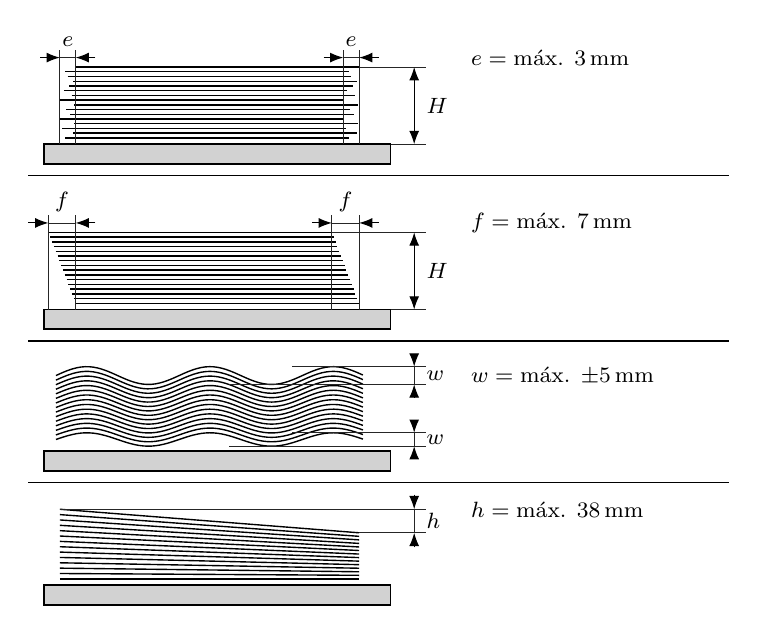
\begin{tikzpicture}[
		>=Latex,
		font=\footnotesize, % 8-9pt estándar IEEE
		dim/.style={<->, >=Latex, line width=0.4pt},
		guide/.style={line width=0.3pt, black!85},
		base/.style={fill=gray!35, draw=black, line width=0.6pt},
		sheet/.style={draw=black, line width=0.5pt},
		annot/.style={font=\footnotesize, anchor=west}
	]

	% ==========================================
	% CASO 1: Desalineación escalonada (e)
	% ==========================================
	\begin{scope}[yshift=0cm]
		\draw[base] (-0.2, 0) rectangle (4.2, 0.25);

		% Hojas apiladas (L = 3.6 cm)
		\foreach \y/\dx in {
				0.33/-0.13,
				0.39/-0.03,
				0.45/-0.17,
				0.51/-0.02,
				0.57/-0.20,
				0.63/-0.07,
				0.69/-0.12,
				0.75/-0.02,
				0.81/-0.20,
				0.87/-0.05,
				0.93/-0.15,
				0.99/-0.08,
				1.05/-0.03,
				1.11/-0.10,
				1.17/-0.13,
				1.23/0.00
			}{
				\draw[sheet] (0.20 + \dx, \y) -- (3.80 + \dx, \y);
			}

		% Cota e izquierda
		\draw[guide] (0.00, 0.25) -- (0.00, 1.45);
		\draw[guide] (0.20, 0.25) -- (0.20, 1.45);
		\draw[guide] (0.00, 1.35) -- (0.20, 1.35);
		\draw[->, >=Latex, line width=0.4pt] (-0.25, 1.35) -- (0.00, 1.35);
		\draw[->, >=Latex, line width=0.4pt] (0.45, 1.35)  -- (0.20, 1.35);
		\node[above=0.5pt] at (0.10, 1.35) {\(e\)};

		% Cota e derecha
		\draw[guide] (3.60, 0.25) -- (3.60, 1.45);
		\draw[guide] (3.80, 0.25) -- (3.80, 1.45);
		\draw[guide] (3.60, 1.35) -- (3.80, 1.35);
		\draw[->, >=Latex, line width=0.4pt] (3.35, 1.35) -- (3.60, 1.35);
		\draw[->, >=Latex, line width=0.4pt] (4.05, 1.35) -- (3.80, 1.35);
		\node[above=0.5pt] at (3.70, 1.35) {\(e\)};

		% Cota de altura H
		\draw[guide] (3.80, 1.23) -- (4.65, 1.23);
		\draw[guide] (4.20, 0.25) -- (4.65, 0.25);
		\draw[dim] (4.50, 0.25) -- (4.50, 1.23) node[midway, right=1pt] {\(H\)};

		% Texto IEEE
		\node[annot] at (5.10, 1.35) {\(e = \text{máx. \qty{3}{\mm}}\)};[cite: 1]
		\draw[line width=0.5pt] (-0.4, -0.15) -- (8.5, -0.15);
	\end{scope}

	% ==========================================
	% CASO 2: Inclinación lateral / sesgo (f)
	% ==========================================
	\begin{scope}[yshift=-2.1cm]
		\draw[base] (-0.2, 0) rectangle (4.2, 0.25);

		\foreach \i in {0,...,15}{
				\pgfmathsetmacro{\y}{0.33 + \i*0.06}
				\pgfmathsetmacro{\xi}{0.20 - \i*0.023}
				\pgfmathsetmacro{\xd}{3.80 - \i*0.023}
				\draw[sheet] (\xi, \y) -- (\xd, \y);
			}

		% Cota f izquierda
		\draw[guide] (-0.145, 0.25) -- (-0.145, 1.45);
		\draw[guide] (0.20, 0.25)   -- (0.20, 1.45);
		\draw[guide] (-0.145, 1.35) -- (0.20, 1.35);
		\draw[->, >=Latex, line width=0.4pt] (-0.40, 1.35) -- (-0.145, 1.35);
		\draw[->, >=Latex, line width=0.4pt] (0.45, 1.35)  -- (0.20, 1.35);
		\node[above=0.5pt] at (0.027, 1.35) {\(f\)};

		% Cota f derecha
		\draw[guide] (3.455, 0.25) -- (3.455, 1.45);
		\draw[guide] (3.80, 0.25)  -- (3.80, 1.45);
		\draw[guide] (3.455, 1.35) -- (3.80, 1.35);
		\draw[->, >=Latex, line width=0.4pt] (3.20, 1.35) -- (3.455, 1.35);
		\draw[->, >=Latex, line width=0.4pt] (4.05, 1.35) -- (3.80, 1.35);
		\node[above=0.5pt] at (3.627, 1.35) {\(f\)};

		% Cota H
		\draw[guide] (3.455, 1.23) -- (4.65, 1.23);
		\draw[guide] (4.20, 0.25)  -- (4.65, 0.25);
		\draw[dim] (4.50, 0.25) -- (4.50, 1.23) node[midway, right=1pt] {\(H\)};

		\node[annot] at (5.10, 1.35) {\(f = \text{máx. \qty{7}{\mm}}\)};[cite: 1]
		\draw[line width=0.5pt] (-0.4, -0.15) -- (8.5, -0.15);
	\end{scope}

	% ==========================================
	% CASO 3: Ondulación / Curvatura (w)
	% ==========================================
	\begin{scope}[yshift=-3.9cm]
		\draw[base] (-0.2, 0) rectangle (4.2, 0.25);

		\foreach \i in {0,...,14}{
				\pgfmathsetmacro{\ybase}{0.40 + \i*0.058}
				\pgfmathsetmacro{\amp}{0.085 + \i*0.002}
				\draw[sheet, domain=-0.05:3.85, samples=75, smooth]
				plot (\x, {\ybase + \amp*sin((\x + 0.05) * 230)});
			}

		% Cota w superior
		\draw[guide] (2.95, 1.325) -- (4.65, 1.325);
		\draw[guide] (2.15, 1.100) -- (4.65, 1.100);
		\draw[guide] (4.50, 1.100) -- (4.50, 1.325);
		\draw[->, >=Latex, line width=0.4pt] (4.50, 1.48) -- (4.50, 1.325);
		\draw[->, >=Latex, line width=0.4pt] (4.50, 0.94) -- (4.50, 1.100);
		\node[right=1pt] at (4.50, 1.21) {\(w\)};

		% Cota w inferior
		\draw[guide] (2.95, 0.485) -- (4.65, 0.485);
		\draw[guide] (2.15, 0.315) -- (4.65, 0.315);
		\draw[guide] (4.50, 0.315) -- (4.50, 0.485);
		\draw[->, >=Latex, line width=0.4pt] (4.50, 0.64) -- (4.50, 0.485);
		\draw[->, >=Latex, line width=0.4pt] (4.50, 0.16) -- (4.50, 0.315);
		\node[right=1pt] at (4.50, 0.40) {\(w\)};

		\node[annot] at (5.10, 1.21) {\(w = \text{máx. \qty{+-5}{\mm}}\)};[cite: 1]
		\draw[line width=0.5pt] (-0.4, -0.15) -- (8.5, -0.15);
	\end{scope}

	% ==========================================
	% CASO 4: Inclinación en cuña (h)
	% ==========================================
	\begin{scope}[yshift=-5.6cm]
		\draw[base] (-0.2, 0) rectangle (4.2, 0.25);

		\foreach \i in {0,...,13}{
				\pgfmathsetmacro{\yl}{0.33 + \i*0.068}
				\pgfmathsetmacro{\yr}{0.33 + \i*0.045}
				\draw[sheet] (0.0, \yl) -- (3.8, \yr);
			}

		% Cota h
		\draw[guide] (0.00, 1.214) -- (4.65, 1.214);
		\draw[guide] (3.80, 0.915) -- (4.65, 0.915);
		\draw[guide] (4.50, 0.915) -- (4.50, 1.214);
		\draw[->, >=Latex, line width=0.4pt] (4.50, 1.40) -- (4.50, 1.214);
		\draw[->, >=Latex, line width=0.4pt] (4.50, 0.73) -- (4.50, 0.915);
		\node[right=1pt] at (4.50, 1.065) {\(h\)};

		\node[annot] at (5.10, 1.21) {\(h = \text{máx. \qty{38}{\mm}}\)};[cite: 1]
	\end{scope}

\end{tikzpicture}
\end{document}

	\caption{Criterios y tolerancias geométricas para el apilado.}
	\label{fig:criterios_apilado}
\end{figure}



% \section{LGAC en la que se enmarca el proyecto}
% \section{Objetivo general}
% \section{Objetivos específicos}
% \section{Alcances y delimitaciones}
% \section{Justificación}
